In this final lecture of part 1 of the course we study a part of the political process which we have so far left untouched, namely the politics that happen after an election has taken place. In a case with non-perfect affection of politicians, the elected will have positions and policies to bargain for, in favor of themselves or their supporters.

We still consider the question of how much governments should spend ($g$) but now we consider the bargaining game that takes place after politicians are elected. To give politicians different preferences for $g$ we assume they vary in income. We can interpret this either as egoistic citizen candidates or as politicians representing different population groups which vary in $y$.
\\ \\
Specifically consider three politicians $L,M,R$ and their incomes which are ranked $y^L < y^M < y^R$ and assume their preferences are given by $w^J=c^J + H(g)$. Each candidates preferred policy is then 
\begin{equation}
    g^J = H_g^{-1}(y^J / y)
\end{equation}
implying $g^L > g^M > g^R$ because $H_g^{-1}$ is decreasing in its argument.

\paragraph{One round bargaining} We take as a given a specific protocol for bargaining, in this first case assume that nature selects a politician $a\in[L,M,R]$ to be agenda setter. This individual proposes a policy $g_a$ as a take-it-or-leave-it offer. If two politicians agree on $g_a$ it is accepted, but if only one (or 0) candidates support $g_a$ some status quo policy $\bar{g}$ is implemented instead.

First assume $a=M$ and that in this case the proposer suggests $g_a=g^M$ and since $M$ is the median voter in the legislature (not the population) this proposal is the Condorcet winner and passes. Why? Both of the two other politicians $L,R$ cannot both at the same time support any other policy $\tilde{g}$ over $g^M$, as their ranking means one of them will always prefer $g_M$. Now knowing this it is obvious that $M$ will play $g^M$ to begin with.
\\ \\
While $a=M$ is trivial, next consider the case where $a=L$. Now the optimal decision for $L$ depends on the value of $\bar{g}$.
\begin{itemize}
    \item If $\bar{g}>g^L$ the proposer should suggest $g^L$ which passes unanimously as everybody prefer this to the status quo. 
    \item If $g^M \leq \bar{g} \leq g^L$ he should propose $\bar{g}$, this too passes unanimously as it is identical to the outside option. 
    \item If $\bar{g} \leq g^M$ he should propose $\min[g^L, \tilde{g}^M]$ where $\tilde{g}^M$ is set such that $W^M(\tilde{g}^M)=W^M(\bar{g})$, that is $\tilde{g}^M$ is as bad as the outside option to the median politician, but no worse. This ensures $M$ agrees to the policy.
\end{itemize}
Notice that in all cases $M$ is part of the coalition, so while the median politician is not completely determining the outcome, the median politicians position but bounds on what proposals are possible to make by $L$ or $R$. Furthermore the possibilities for $L$ and $R$ depend heavily on the value of $\bar{g}$.

\paragraph{Two round bargaining} Now lets extend our reasoning to two round bargaining. In the first round everything goes as previously, except if $g_a$ fails, a new random agenda setter $a_2 \neq a_1$ is selected, to propose a new policy $g_2$. Then if no agreement is reached in the second round the legislature implements $\bar{g}$. Otherwise $g_2$ will be implemented. The logic is the same as in the single round case, except the bounds of what can be offered to $M$ is now not $W^M(\bar{g})$, but the \textit{continuation value} for $M$ from going on to a second round.

Say $L$ is the proposer, this means $L$ should propose $g\in[g^M, g^L]$ such that $g$ is equal to the continuation value of $M$. This ensures the proposal passes with support from $M$. If the continuation value increases, this forces $L$ to propose a $g$ closer to $g^M$.

\subsection{Multilateral bargaining \citep{baron_bargaining_1989}} 
Consider a legislature with $n$ single vote members, who each represents a district from which they were elected. The game considered by \cite{baron_bargaining_1989} is then a kind of divide-the-dollar game where the legislature bargains to distribute a fixed amount of resources.
This problem has $n-1$ dimensions, i.e. the number of districts among which to divide the resource, except for the last district in which the amount of resource is residually given. Thus no condorcet winner generally exists, and instead majority voting results in condorcet cycles. To give some structure the idea is therefore to alter the assumptions on the aggregation of preferences to something different than majority voting. In particular the proposed structure is a legislature with a set of rules
\begin{itemize}
    \item[1.] A recognition rule, which determines who in the legislature can propose policy.
    \item[2.] An amendment rule, that sets up rules for making changes to the initial proposal. 
    \item[3.] A voting rule, which decides how voting is conducted and in particular what is required for a proposal to pass. 
    \item[4.] A deadline rule, setting the maximum number of bargaining rounds before an outside option is adopted.  
\end{itemize}
A very simple set of such rules could be 1) equal probability of every legislator being selected as proposer 2) No amendments allowed 3) Majority rule and 4) Two sessions of bargaining. In this setup some random member $P_1$ is selected as proposer and proposes a distribution 
\begin{equation}
    x^{P_1} = (x_1^{P_1},...,x_n^{P_1})
\end{equation}
such that $\sum x_i \leq 1$. If a majority approves the proposal it becomes policy, otherwise a second round of bargaining is begin. If a majority still doesn't agree with the proposal the status quo $x^{SQ}=(0,...,0)$ is implemented.
\\ \\ 
We assume that a members payout of a result in round $t$ is $\delta^t x_i$ where $\delta$ is some kind of common discount factor that measures the "cost of delay". This ensures some bias towards finishing the game early. 
\begin{SCfigure}[][h]
    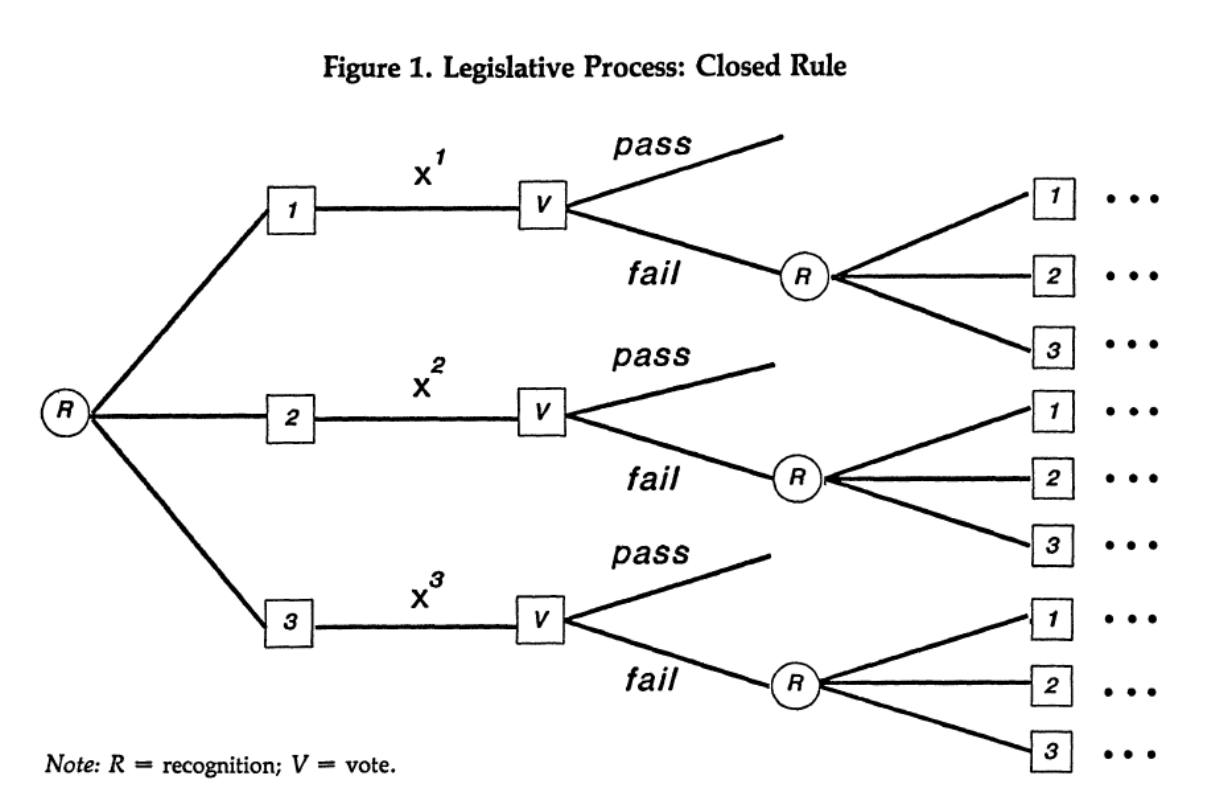
\includegraphics[width=0.6\textwidth]{figures/bf.png}
    \caption{\textbf{Figure 1 from \cite{baron_bargaining_1989}} showing the structure of the closed rule game.}
\end{SCfigure}
The model can be solved by backwards induction. In the last period the continuation value for everyone is $0$ so in this vote any voter will vote in favor of a distribution as long as it yields a small positive payoff. From the perspective of the proposer only $(n-1)/2$ votes are needed for the proposal to pass, so the proposer in the second round will propose some small payoff $\epsilon>0$ to $(n-1)/2$ districts and payoff of $0$ for the rest. This leaves the proposer with a value of $\approx 1$ (technicalities about $\epsilon$ withstanding).
\\ \\
In period 1 all legislators know that there is an equal probability $1/n$ of begin selected as proposer in the second round of bargaining, and their continuation value is therefore $\delta/n$. Anticipating this the proposer in period 1 will offer $\delta / n$ to exactly $(n-1)/2$ districts and 0 to the remaining. This leaves the payoff for the proposer $1 - (n-1) \frac{\delta}{2n}$. Thus the equilibrium distribution is 
\begin{equation}
    x^{P_1} = (\underbrace{1-\frac{n-1}{2} \frac{\delta}{n}}_{P_1}, \underbrace{\frac{\delta}{n}, ...,\frac{\delta}{n}}_{(n-1)/2 \text{ players}}, \underbrace{0,..,0}_{\text{remaining } (n-1)/2})
\end{equation}
which passes with a minimal majority. Notice that there are no veto players as the proposer can propose any of a whole set of equilibria in which different districts get 0. Furthermore we see quite a significant benefit from being awarded the initial proposer role. This is in part a result of the majority rule system, as the proposer can skim a benefit from the minority and in part because of the no-amendments rule which prevents modifying the proposal by $P_1$. Furthermore the closed rule model always have a solution in the first round meaning no delays.

\subsection{Empirical evidence for the bargaining model \citep{ansolabehere_voting_2005}}
The paper by \citeauthor{ansolabehere_voting_2005} tests aspect of the model by \citeauthor{baron_bargaining_1989}. Especially they test the theoretical observation that the proposer will gain a disproportionate gain from the bargaining. They do this in the setting of government formation. In this setting the prediction is that the formateur of the government should get a disproportionate amount of cabinet seats in the finished government. 
\\ \\ 
An important part of the paper is the use of "minimum-integer voting weights" instead of raw seat shares in the respective parliament. This is essentially a mapping from the parliament seats to a measure of the number of possible coalitions a given party can be in to form a majority. In particular it is the minimum number of legislators each party could have while preserving the possible coalitions (without respect to the total size of parliament). The reason for this conversion is that while seat share and minimal-integer weight shares are correlated, the latter are a better measure of a political partys bargaining potential. Furthermore the theory is more accurately mirrored by minimal-integer voting weights than party seat shares. Notice the simple version of the \citeauthor{baron_bargaining_1989} does not include parties, but this extension is simple to implement, and predicts that parties with high voting weights get high bargaining power, that the formateur enjoys agenda power and overproportional placement in the government. Importantly alternative models does not provide the second implication, but instead predict proportional representation for all parties regardless of their role in the bargaining process.

\begin{SCfigure}[][h]
    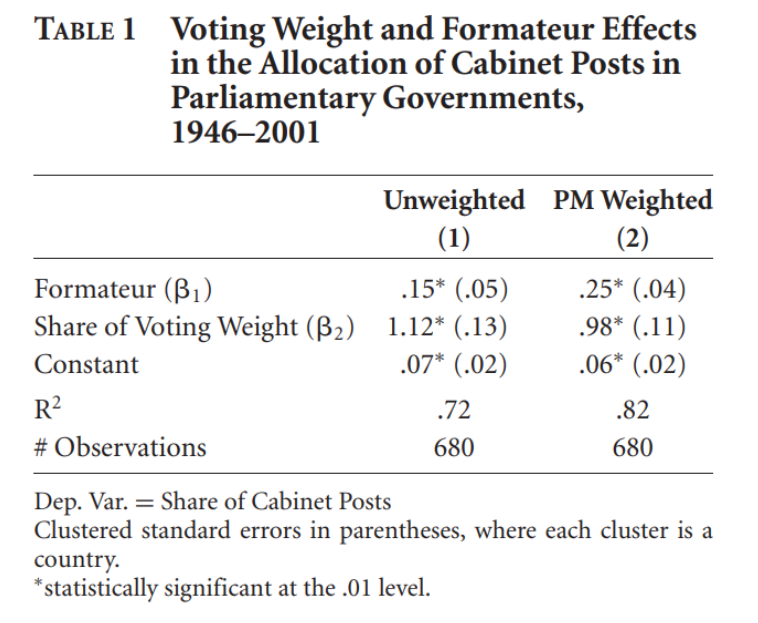
\includegraphics[width=0.6\textwidth]{figures/ansolres.png}
    \caption{\textbf{Key results from \cite{ansolabehere_voting_2005}}}
\end{SCfigure}

The table shows results from regressing the number of cabinet posts awarded to each party on a dummy for being the formateur party as well as their share of voting weights. Their results are significant and suggest a formateur disproportionate advantage in accordance with the models predictions. Importantly studies that use seat shares instead of voting weights does not reach the same conclusion. 